%% =====================================================================
%% Replicating a paper --- course template (SSRN format)
%% ML & FinTech, National Yang Ming Chiao Tung University
%% Instructor: Huei-Wen Teng
%%
%% Condensed to the 2,400-word limit. The uncondensed version is main-full.tex.
%% Every instruction to you is written in \emph{italics} using \inst{...}.
%% Delete each instruction once you have acted on it.
%% =====================================================================

\documentclass[12pt]{article}

\usepackage{adjustbox,array,amssymb,amsmath,amsfonts,eurosym,geometry,graphicx,
            caption,color,setspace,sectsty,comment,footmisc,natbib,pdflscape,
            subfigure,longtable,lscape,float,multirow,booktabs,makecell,
            hyperref,ulem,appendix}

\normalem
\onehalfspacing

\newtheorem{theorem}{Theorem}
\newtheorem{corollary}[theorem]{Corollary}
\newtheorem{proposition}{Proposition}
\newenvironment{proof}[1][Proof]{\noindent\textbf{#1.} }{\ \rule{0.5em}{0.5em}}

\newtheorem{hyp}{Hypothesis}
\newtheorem{subhyp}{Hypothesis}[hyp]
\renewcommand{\thesubhyp}{\thehyp\alph{subhyp}}

\newcolumntype{L}[1]{>{\raggedright\let\newline\\arraybackslash\hspace{0pt}}m{#1}}
\newcolumntype{C}[1]{>{\centering\let\newline\\arraybackslash\hspace{0pt}}m{#1}}
\newcolumntype{R}[1]{>{\raggedleft\let\newline\\arraybackslash\hspace{0pt}}m{#1}}

\geometry{left=1.0in,right=1.0in,top=1.0in,bottom=1.0in}

%% ---------------------------------------------------------------------
%% Instructions are italic. Delete the \inst{...} once you have done it.
%% ---------------------------------------------------------------------
\newcommand{\inst}[1]{\textit{#1}}

\begin{document}

\begin{titlepage}

\title{Replicating the paper:
       Temporal Relational Ranking for Stock Prediction \citep{feng2019temporal}}

\author{Yue Zhen Huang\thanks{Department of Information Management and Finance,
        National Yang Ming Chiao Tung University. Email:
        \inst{your NYCU email, as \texttt{name@nycu.edu.tw}}.}}

\date{\today}
\maketitle

\begin{abstract}
\noindent
Stock returns are usually predicted from each stock's own history, although firms linked
through an industry, a supply chain, or shared fund holdings tend to move together.
\citet{feng2019temporal} address this with Relational Stock Ranking (RSR), which passes
information between related stocks through a graph convolution over a fixed relation graph and
ranks stocks by next-day return. This replication reproduces RSR on the paper's NASDAQ data and
adds a test the original does not run: a relation graph re-estimated from rolling 60-day return
correlations instead of held fixed, motivated by our finding that the share of related stock
pairs varies six- to seven-fold across windows. At a matched, converged training budget, neither
the static nor the dynamic graph lowers mean-squared error relative to a relation-blind baseline,
so the original claim does not replicate in our setting. The dynamic model's ranking flips from
best at 10 epochs to worst at 50, and after we correct a window-alignment bug it beats both
alternatives on simulated trading return while trailing the baseline on top-1 ranking accuracy.
We are interested in whether the strength of a relation, and not only its existence, carries
predictive information.

\vspace{0in}
\noindent\textbf{Keywords:} Stock Prediction, Learning to Rank, Graph-based Learning

\vspace{0in}
\noindent\textbf{JEL Codes:} G17, C45, C53\footnote{\citet{feng2019temporal} do not report JEL
codes, so we chose these ourselves from the JEL classification system: G17 (Financial
Forecasting and Simulation), C45 (Neural Networks and Related Topics), and C53 (Forecasting and
Prediction Methods; Simulation Methods).}

\bigskip
\end{abstract}

\setcounter{page}{0}
\thispagestyle{empty}
\end{titlepage}
\pagebreak

\newpage
\clearpage


\section{Motivation}
\label{sec:motivation}

A stock's future return is usually modeled from its own history, which discards information that
is easy to observe: companies in the same industry, supply chain, or fund tend to move together,
because a shock to one is often a shock to the group. Empirical finance shows that information
travels along such links and reaches prices with a delay: customer and supplier industries
cross-predict each other's returns \citep{menzly2010market}, news about economically linked firms
is priced slowly \citep{cohen2008economic}, and money managers' commodity-futures positions predict
producers' stock returns the following week \citep{ho2023smart}. Links also shape real outcomes and
differ in strength: upstream tariff cuts raise downstream investment
\citep{martin2024downstream}, and shared institutional owners lengthen supply-chain relationships
\citep{freeman2025overlapping}. \citet{feng2019temporal} address this with
Relational Stock Ranking (RSR). A graph of relations between stocks (shared industry, and
Wikidata facts on ownership, supply, and competition) enters a Temporal Graph Convolution layer on
top of an LSTM encoding of each stock's price history. The model is trained to rank stocks by
next-day return rather than to regress it, since a top-$k$ trading strategy cares about relative
order more than exact values.

This project replicates RSR on the paper's NASDAQ universe and industry graph, then asks what the
original does not: what if the relation graph is not fixed? RSR builds its graph once, from
static facts. The \emph{strength} of a relation, however, is not static: two firms in one sector
can move in lockstep under a shared macro shock and decouple once it passes, and a supply-chain
tie can matter around an earnings announcement and not the rest of the year. On this dataset,
rolling 60-day return correlations show the share of related stock pairs swinging six- to
seven-fold between windows (Section~\ref{sec:data}). If that variation carries information a
static graph misses, a model blind to it leaves something on the table.

\subsection{Research questions}

\begin{itemize}
  \item \textbf{RQ1 (replication).} Does a static relation graph, as in \citet{feng2019temporal},
  improve next-day return ranking relative to a baseline that treats stocks independently?
  \item \textbf{RQ2 (extension).} Does re-estimating the graph over rolling windows improve
  ranking further, relative to both the baseline and the static-relation model?
\end{itemize}

\subsection{Contribution}

We replicate the baseline and RSR on the official NASDAQ data and add a third model, identical to
RSR except that the relation graph is a time-indexed input rather than a training-time constant,
so any difference from static RSR isolates the effect of letting the graph change. At convergence,
neither graph lowers mean-squared error relative to the baseline, so RQ1 is not supported. For
RQ2, once a window-alignment bug is fixed (Section~\ref{sec:results}), the dynamic model beats
both alternatives on simulated trading return but trails the baseline on top-1 ranking accuracy.
We report this split result, and an earlier reversal between short and converged runs, as
findings rather than failed experiments.

\subsection{Related work}
\label{sec:related}

\citet{cui2023temporal} extend relation-based prediction from pairwise relations to group-wise
hypergraphs (industry-belonging and fund-holding) with hierarchical attention, and
\citet{jafari2022gcnet} apply a graph convolutional network to a stock-relation graph; their code
is withheld, so we treat it as a design reference, not a reproducible baseline. Like RSR, both
fix which stocks are related for the whole of training. Empirical finance suggests such channels
vary over time: \citet{evgeniou2023uncovering} find that firm-level return predictability is
sparse and heterogeneous, shifting across firms and periods, which motivates estimating relation
strength period by period. Deep learning has also entered cross-sectional asset pricing:
\citet{feng2024deep} generate latent risk factors with a network trained on firm characteristics.

\inst{TODO: the template asks for five fundamental and five machine-learning papers, and both
sets are now cited. Read every cited paper before submission: a citation you have not read does
not belong here, and the descriptions above rest on abstracts.}


\section{Data}
\label{sec:data}

We use the NASDAQ portion of the dataset released with \citet{feng2019temporal}: daily features
for 1{,}026 tickers over 1{,}246 trading days, and a static industry graph. The repository
describes its raw pull as thirty years of data on more than 8,000 stocks, but the modeling sample
is roughly five years, and only 1{,}026 stocks survive the paper's liquidity and history filters.

\subsection{Dependent and independent variables}

\begin{itemize}
  \item \textbf{Response (continuous).} The next-day return of each stock, which the models
  predict and rank across stocks.
  \item \textbf{Predictors (continuous).} For each stock and day: the 5-, 10-, 20-, and 30-day
  moving averages of the close price and the close-to-close return ratio, each normalized by the
  stock's maximum price over the sample.
  \item \textbf{Relation graph (binary).} A $1{,}026\times1{,}026$ one-hot encoding of shared
  membership across 97 industry categories.
\end{itemize}

\inst{TODO: give each variable an acronym and check that the response definition above matches
the original paper. The dataset is the one released with the original paper, so it is not
expected to differ; say so explicitly if that is right.}

\subsection{Data exploration, cleaning and preprocessing}

Exploratory analysis (notebook \texttt{eda.ipynb}) found two gaps between the data and its
documentation.

\begin{enumerate}
  \item \textbf{Missing values are not \texttt{NaN}.} The pipeline (\texttt{preprocess/eod.py})
  pads missing trading days with a sentinel of $-1234$. Left in, it drives raw skewness to about
  $-23$ for every feature column; stripped, skewness is an unremarkable $-0.3$ to $-0.4$. The
  $-23$ is an artifact of an undocumented missing-value code, not a property of prices.
  \item \textbf{The relation graph includes non-company tickers.} 156 of the 1{,}026 tickers
  (15.2\%) have industry \texttt{"n/a"}; they are ETFs and index funds (e.g.\ \texttt{QQQ},
  \texttt{SHV}) whose return is a basket average with no industry relation, and 17 of them are
  isolated in the graph.
\end{enumerate}

Every model treats the sentinel as missing. For consistency across the static and dynamic
conditions, all keep the 156 tickers in the universe; removing them is an open item in the project
progress notes (\texttt{PROGRESS.md}).

To test whether the graph is really static, we compute rolling 60-day return correlations and
binarize each window at $|\text{corr}|>0.5$. Across the 21 non-overlapping windows, edge density
(the share of stock pairs counted as related) ranges from 3.6\% to 22.5\% (Table~\ref{tab:density}).
A static graph cannot approximate that.

\begin{table}[h]
\centering
\caption{Edge density of the rolling-correlation relation graph, selected 60-day windows
(NASDAQ, 1{,}026 tickers, $|\text{corr}|>0.5$).}
\label{tab:density}
\begin{tabular}{lccccc}
\toprule
Window & 0 & 4 & 14 & 19 & 20 \\
\midrule
Edge density & 3.6\% & 11.5\% & 22.5\% & 4.6\% & 4.2\% \\
\bottomrule
\end{tabular}
\end{table}


\section{Methodology}
\label{sec:methods}

We compare three models on the same universe, features, next-day ranking objective, optimizer
(Adam), and date split (indices 0--755 / 756--1007 / 1008-- of the 1{,}246 days). All use
$\text{seq}=4$ and $\text{unit}=32$ and the same combined loss: mean-squared error on predicted
return, plus a pairwise ranking penalty for stock pairs whose predicted order contradicts their
realized order, weighted by $\alpha$.

\subsection{Benchmark model}

\textbf{Baseline: Rank\_LSTM.} A single-layer LSTM encodes each stock's own history and predicts
next-day return from the final hidden state, with no information exchanged between stocks. This is
the ``stocks are independent'' benchmark that RSR is designed to beat.

\textbf{RSR: static relation graph.} RSR takes the baseline LSTM's learned embedding, exported
after training because the authors' pretrained file is only available through an external link,
and propagates it over the static industry graph with softmax-normalized attention over each
stock's neighbors. It then combines the propagated and original representations into the final
prediction. The graph is a training-time constant.

\subsection{Experimental Design}

Figure~\ref{fig:flow} shows the procedure from raw data to the reported test-set numbers.

\begin{figure}[htbp]
\centering
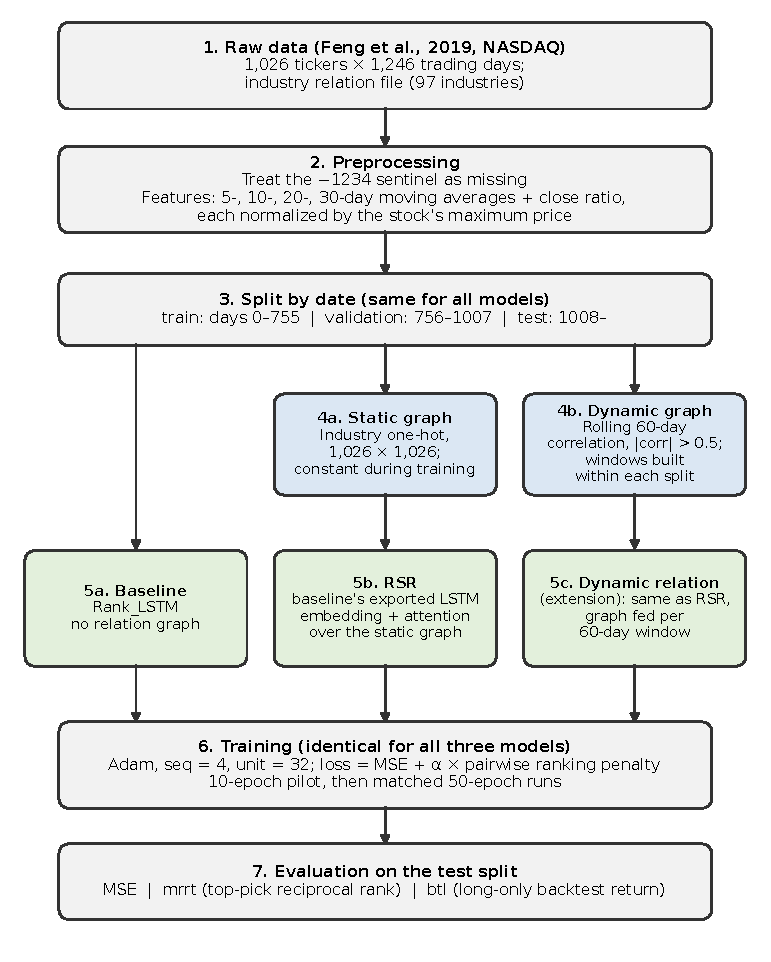
\includegraphics[width=0.88\textwidth]{figures/flowchart.pdf}
\caption{Experimental design, from raw data to reported test-set metrics. The
``unaligned windows'' variant in Table~\ref{tab:results-aligned} differs from box 4b only in
that its windows are built over the full sample instead of within each split.}
\label{fig:flow}
\end{figure}

\textbf{Extension: dynamic relation graph.} The extension is identical to RSR except that the
graph is fed at each training step instead of being a constant: it is the rolling-correlation
graph for the 60-day window containing the current date (\texttt{preprocess/dynamic\_relation.py}).
Everything else is held fixed, so any difference from static RSR isolates the effect of letting
the graph vary over time.

\subsection{Performance measures}

On the test split we report \emph{MSE}; \emph{mrrt}, the mean reciprocal rank of the true
top-return stock (higher means the model's top pick is more often the actual best); and
\emph{btl}, the simulated return of a long-only strategy that buys the top-ranked stock each day.


\section{Results}
\label{sec:results}

\inst{TODO: put your numbers and the original paper's numbers side by side in one table. The
tables below report only this replication's own runs.}

\subsection{An early result that did not survive convergence}

RSR is far costlier to train than the baseline, since attention runs over the full
$1{,}026\times1{,}026$ relation matrix at every step, so we first compared all three models at a
reduced budget of 10 epochs. There the dynamic model led both alternatives on both ranking metrics
(mrrt $0.048$ vs.\ $0.038$ baseline and $0.042$ RSR; btl $0.87$ vs.\ $0.67$ and $0.48$), which
read as support for RQ2.

\subsection{Results at matched convergence (50 epochs)}

\begin{table}[h]
\centering
\caption{Test-set performance, all three models trained to 50 epochs on the same NASDAQ universe
and embedding.}
\label{tab:results50}
\begin{tabular}{lccc}
\toprule
Model & Test MSE & Test mrrt & Test btl \\
\midrule
Baseline (Rank\_LSTM, no relation) & 0.0003774 & \textbf{0.0488} & 1.018 \\
RSR (static industry relation) & 0.0003774 & 0.0276 & \textbf{1.130} \\
Dynamic relation (this project) & 0.0003778 & 0.0288 & 0.861 \\
\bottomrule
\end{tabular}
\end{table}

At 50 epochs (Table~\ref{tab:results50}) the picture changes in two ways. First, MSE is essentially
identical across models: the baseline and static RSR agree to seven decimal places and the dynamic
model is 0.1\% higher, so RQ1 is not supported. Second, the dynamic model's ranking advantage
reverses. The baseline has by far the highest mrrt (0.049 vs.\ 0.028--0.029), static RSR the
highest btl (1.13 vs.\ 0.86), and the dynamic model is the worst performer on both.

\subsection{Why the early signal did not hold}

We considered three explanations. (1) The rolling correlation is a high-variance statistic, and a
single fixed threshold discards magnitude information. (2) The 60-day windows ignored the
train/validation/test boundaries, so one window's graph could span a split. (3) The static graph
may already suffice at this scale, leaving little room for a time-varying signal net of its noise.

Only (2) is fixable without a new modeling choice, so we rebuilt the windows separately within
each split (\texttt{preprocess/dynamic\_relation.py}) and made the model look up each date's
window from the resulting boundaries. Retraining for 50 epochs (Table~\ref{tab:results-aligned})
raises the dynamic model's btl from the lowest of the three (0.861) to the highest (1.214) and its
mrrt from 0.0288 to 0.0311, still below the baseline's 0.0488; MSE is essentially unchanged. A
construction flaw unrelated to whether time-varying relations carry information had made the
dynamic model look worse than it is.

\begin{table}[h]
\centering
\caption{Test-set performance, dynamic-relation model before and after aligning window
boundaries to the train/validation/test split (50 epochs; baseline and RSR rows repeated from
Table~\ref{tab:results50} for comparison).}
\label{tab:results-aligned}
\begin{tabular}{lccc}
\toprule
Model & Test MSE & Test mrrt & Test btl \\
\midrule
Baseline (no relation) & 0.0003774 & \textbf{0.0488} & 1.018 \\
RSR (static relation) & 0.0003774 & 0.0276 & 1.130 \\
Dynamic relation, unaligned windows & 0.0003778 & 0.0288 & 0.861 \\
Dynamic relation, split-aligned windows & 0.0003776 & 0.0311 & \textbf{1.214} \\
\bottomrule
\end{tabular}
\end{table}

\subsection{Did the replication succeed?}

Not in the direction \citet{feng2019temporal} report. Their central claim is that relational
information lowers prediction error and improves ranking; at convergence we find neither. We see
three non-exclusive reasons, none of which a single run can settle. (i) We did not tune
hyperparameters: $\text{seq}=4$ and $\text{unit}=32$ were chosen for consistency, while the
original paper's wikidata run uses $\text{seq}=16$ and $\text{unit}=64$. (ii) Every number comes
from one run with one seed, so the ranking between models may not be stable. (iii) The embedding
was exported from our own baseline run, not the authors' released artifact. The robustness checks
in \texttt{PROGRESS.md} (a second seed and a brief hyperparameter sweep) are not yet done.

\subsection{Interpreting the dynamic-relation result}
\label{sec:discussion}

Once the alignment is fixed, RQ2 is no longer a clean no: the dynamic model beats the baseline
and static RSR on btl (1.214 vs.\ 1.018 and 1.130) but trails the baseline on mrrt (0.031 vs.\
0.049). One reading is that a time-varying graph tells the model which \emph{groups} of stocks are
moving together in a period, which helps a strategy that overweights several top names, while
adding pairwise noise that hurts a metric rewarding only the single best pick. We have no
evidence for this beyond the two numbers.

The result does not show that industry relations or correlation-based dynamic relations are
generally better. It shows that this construction, with one window length (60 days) and one
threshold ($|\text{corr}|>0.5$), neither tuned, wins on one metric and loses on another. Shrinkage
instead of a hard threshold, continuous instead of block updates, or dynamics layered on top of the
industry graph could shift that balance. Results are also for NASDAQ and the industry graph only
(the original paper also reports a Wikidata condition), with the 156 ETF and fund tickers left in
the graph.


\section{Conclusion}
\label{sec:conclusion}

We replicated \citet{feng2019temporal}'s RSR on its official NASDAQ data and extended it with a
dynamic relation graph estimated from rolling 60-day correlations. At a matched, converged budget,
neither the static nor the dynamic graph lowered mean-squared error relative to a relation-blind
baseline. The dynamic model's standing on the other two metrics reversed twice: best at 10 epochs,
worst at 50, and, after fixing the window-alignment bug, ahead of both alternatives on trading
return while still behind the baseline on top-1 ranking accuracy. Two lessons carry beyond this
comparison. An early-training read is not a safe substitute for a matched-budget comparison when
the models differ in cost, and a preprocessing detail with no visible link to the architecture, how
a rolling window is chopped relative to a data split, can produce a result that reads as a finding
about the model.

The next steps are the robustness checks in \texttt{PROGRESS.md}, a second seed and a construction
less dependent on one correlation threshold, together with the open question of why the aligned
dynamic graph helps a portfolio-style metric (btl) but hurts a single-pick one (mrrt). Extending
the comparison to the Wikidata relation and to NYSE, both in the same dataset but not run here,
comes after that.


\section*{Declaration}

\subsection*{Declaration of Pedagogical Purpose}

This manuscript is prepared as part of the course project for Machine Learning and
FinTech at National Yang Ming Chiao Tung University, instructed by Professor
Huei-Wen Teng. The work is intended solely for pedagogical purposes, including
learning, discussion, and academic training. It does not represent original research
submitted for journal publication, nor should it be considered professional financial
advice.

\subsection*{Declaration of generative AI and AI-assisted technologies in the writing process}

\inst{Name the tools you actually used. Replace the bracketed placeholders below.}

During the preparation of this work, the authors used [ChatGPT] and [Grok], developed
by [OpenAI] and [xAI] respectively, in order to improve the clarity, precision, and
overall quality of the writing. After using these tools, the authors reviewed and
edited the content as needed and take full responsibility for the content of the
article.


\bibliographystyle{chicago}
\bibliography{ref}


\appendix

\section{\inst{Appendix title}}

\inst{Titles have to be concise. Put here anything a reader needs in order to
reproduce your work but does not need in order to follow the argument. Delete this
appendix if you have nothing to put in it.}


\end{document}
